\RequirePackage{lineno}
\documentclass[12pt,letterpaper]{article}


\setlength{\textwidth}{6.3in}
\setlength{\textheight}{8.5in}
\setlength{\oddsidemargin}{0.in}
\setlength{\evensidemargin}{0.in}
\setlength{\footskip}{0.5in}


\usepackage{epsfig}
%\usepackage[dvips]{graphicx}
\usepackage{latexsym}
\usepackage{psfig}
\usepackage{colordvi}
\usepackage{fancyhdr}
\usepackage{amssymb}
\usepackage{url}
\usepackage{verbatimbox}
\usepackage{fancyvrb}
%\usepackage{arydshln}
\usepackage{longtable}
%\pagestyle{headings}
\usepackage{rotating}
\usepackage{fancyhdr}
\fancypagestyle{plain}{%
  %            \fancyhead[R]{\fbox{README Sep.2014}}
  \renewcommand{\headrulewidth}{0pt}
}
\usepackage{tikz}
\usetikzlibrary{arrows,shapes,backgrounds}



\begin{document}
\vskip 2.cm
\title{How to run Spectator Tagging Event Generator with the JLab EIC configuration}
\vskip 1.cm
\author{K.~Park$^{1}$\footnote{contact info: parkkj@jlab.org},~C.~E.~Hyde$^{1}$,~D.~Higinbotham$^{2}$\\}
% C.~E.~Hyde$^{1}$, D.~W.~Higinbotham$^{2}$
\maketitle
\begin{center}
$^1$ Old Dominion University, Norfolk, Virginia 23529, USA\\
$^2$ Thomas Jefferson National Accelerator Facility, Newport News, Virginia 23606, USA\\
\end{center}
\vskip 1.cm


\tikzstyle{every picture}+=[remember picture]
\tikzstyle{na} = [baseline=-.1ex]

%\clearpage


\modulolinenumbers[1]
\linenumbers

\abstract{
This is a technical note of the Spectator Tagging Event Generator for broader users. It explains how to compile and run it. 
It also provides an information of download and a very brief description of the source codes. Users can find source at the \textbf{git-Hub} repository with named ``source\_codes2015\_for\_git\_hub.tar.bz''. 
Two given simple scripts ([1] RunSTEG\_PhaseSpace.exe [2] MainRunEIC\_STEG.exe -or- MainRunEIC\_STEG\_Pol.exe) allow users to obtain the simulation outputs (Lund, Ntuples, Roots).
 Through analysis code (user own) with pseudo-data, the neutron structure function is carried out to the on-shell point as a result. At the end of this note, we present our Monte-Calro simulation results as well.
}

\clearpage
\tableofcontents
\clearpage


\section{Introduction}

The JLab Electron-Ion-Collider (EIC) design provides unique capabilities to perform
scattering experiments on polarized light ions (deuterium; ${}^2H$, helium-3; ${}^3He$) with detection 
of forward-moving spectator nucleons (``tagged spectator proton'', $p_S$). Such measurements offer unprecedented 
precision and control of nuclear structure and can definitively address several outstanding questions 
of nuclear physics, such as the quark/gluon structure of the neutron, the modifications by nuclear 
binding in QCD, and the emergence of coherent quark/gluon fields in nuclei~\cite{CWeiss2014}.

The project is running as a Laboratory Directed Research and Development (LDRD) program which meets in to following criteria:
\begin{itemize}
\item{} Conception/preliminary technical analysis of an experimental facility - EIC
\item{} Advanced study of an innovative approach - Spectator Tagging % in high-energy nuclear processes
\item{} Computer modeling, conceptual design and feasibility study - EIC GEMC
\end{itemize}
  
 It develops new methods using the unique strengths of the JLab EIC design with (un)polarized ${}^2H$,
which is the EIC-related R\&D. There is strong demonstrable interest in
the innovative approach in broader users not only JLab but nuclear physics communities.
We have developed a Monte Carlo simulation event generator with both (un)polarized electron and  
(un)polarized deuterium as initial beam energies (5 GeV : 200 GeV, or any combination) in the  collider framework using spectator 
nucleon (either proton or neutron) tagging method.
Monte Carlo events are weighted by any cross-section model which is available in the current market.


This document is a technical note for the Spectator Tagging Event Generator (STEG) and it can be used as an instruction for any user to 
simulate $eD \to e^{\prime} p_S X$ implementing any cross-section model in the EIC framework.
Therefore, we describe a chain of simulation process in following subsections:
\begin{itemize}
\item{} Software repository and directory structure - How to get the software and how it works ?
\item{} Variables definition - What physics variables that code manages
\item{} Set input and Run codes - How to change/select input parameter and run
\item{} Finally, presenting examples of analysis result and incorporation with GEMC
%\item{} Example of the pseudo-data analysis
\end{itemize}


\section{Software}
\subsection{Software repository}
A tar-zip file is available by asking to authors directly or download from the \textbf{git-Hub}.
For the EIC \textbf{git-Hub} website is found ``~\url{https://github.com/JeffersonLab/LightIonEIC/tree/master/Collider}'' and the first release version is available under ~\cite{gitHubLink} repository.\footnote{\Red{The source code should be uploaded with newer version.}}
Once user get the tar file, he/she can un-tar and un-zip file (or un-compress) by ``tar -xvf FileName.tar.gz''. Or one can download all individual source files from the git-Hub repository.

\subsection{Directory structure}
The codes are built with mainly C++ and FORTRAN languages, others are Perl scripts, macros, look-up tables. The codes can be compiled at any computer which has a standard ROOT \underline{version5.34.13} and FORTRAN compilers \underline{f95}. We have compiled and tested on \underline{ifarm65} (CentOS6.5), and \underline{level-2 Jlab Linux} (RedHatEnterprize) machines.~\footnote{Note that the code is not working properly on MacOS for the moment.}
Here is the example of un-tar process. There are few tens of files and four sub-directories will be created:

\fontsize{9}{9}
\begin{Verbatim}[frame=single]
LinuX64> tar -xvf source_codes2015_for_git_hub.tar.bz
LinuX64> cd source_codes2015_for_git_hub_final/

LinuX64> ls                    ; sub-directories
>> ./eic_collider_data/ ; Output from RunSTEG_PhaseSpace.exe
>> ./lund_out/          ; Lund file with cross-section is stored for GEMC run
>> ./ednt10/            ; Ntuple file with cross-section is stored for analysis purpose
>> ./edRootst/          ; Roots file with cross-section is stored for analysis purpose
\end{Verbatim}
\fontsize{12}{12}

The directory contains not only source codes but also run scripts to generate electron-deuterium scattering cross section pseudo-data using either M.~Sargsian's~\cite{MSargsian} or C.~Weiss' model. 

%% It also contains an example of analysis code/script to obtain the extrapolated $F_{2N}$. 
%% \fontsize{7}{7}
%% \begin{Verbatim}[frame=single]
%% LinuX64> ./RunF2D_tPrim_Coll.exe
%% - It calls an analysis code ('mcc_eic.f') and kumac macros/perl scripts.
%% - Fit result can be obtained from ('f2fitcomp.kumac') 
%% \end{Verbatim}
%% \fontsize{12}{12}





\section{Variables definition and Set input parameters}


\subsection{Variables definition}
There are several key physics variables in the code, they are defined by Table~\ref{tab:Variables}. It is important that our  $z$-axis is defined by the direction of the virtual photon. therefore,  $z$-axis is determined in every single event. The cross-sections from model are calculated by Eq.~(\ref{eq:CrossSection}). It provides the integrated cross-section over the recoil nucleon's azimuthal angle $1/(2\pi)$.


\begin{eqnarray}\label{eq:CrossSection}
\frac{d\sigma}{dx dQ^2 (d\alpha_r/\alpha_r) d^2p_{RT}} = factor \times \Big|\psi^{LC}_D(\alpha_R, \vec{p}_{RT})\Big|^2\times F_{2N}(x^{\prime}, Q^2)~,
\end{eqnarray}
where, $x^{\prime}=\frac{x}{2-\alpha_R}$,~$\nu= E_e - E_e^{\prime}$, ~$\psi^{LC}_D(\alpha_R, \vec{p}_{RT})$ is the deuteron light-cone wave function and $F_{2N}(x^{\prime}, Q^2)$ is the nucleon structure function.

\begin{table}[h]
\begin{center}
\begin{tabular}{|c|c|c|}
%\multicolumn{4}{c}{\bf Kinematic binning} \\ \hline
\multicolumn{3}{c}{} \\ 
\hline
{\bf variable} &{\bf definition} &{\bf - }  \\ \hline\hline
$x_{BJ}$ & the momentum fraction carried by & \\
        & an inclusively observed particle &  $ Q^2/(2m_N \nu)$ \\ \hline
$Q^2$ & the squared four momentum transfer &   $2E_eE_e^{\prime}(1-\cos\theta_e)$\\ \hline
$s_e$ & invariant energy square of $e$ and $d$ system & $(k_e + p_d)^2$    \\ \hline
$s_q$ & invariant energy square of $q$ and $d$ system & $(q + p_d)^2$   \\ \hline
$\alpha_R$ & the light-cone momentum fraction of the &   \\
           & deuteron carried out by recoil nucleon & $2(E_r - p_{r}^z)/(E_d - p_{d}^z)$    \\ \hline
$p_{RT}$ & transverse component of the recoil nucleon vs. $q$& GeV   \\ \hline
$-t$ & the invariant momentum transferred   &   \\ 
 & to the recoil nucleon  &  $(p_d - p_r)^2$  \\ \hline
$-t^{\prime}$ & $M_N^2 - t$  & GeV$^2$   \\ \hline
 $Pol_e$, $Pol_d$  & beam polarization of electron, deuteron& \%  \%   \\ \hline
\end{tabular}\\
\caption[Kinematic Variables]{\label{tab:Variables} Kinematic variables}
\end{center}
\end{table}




\subsection{How to work}
Overall, the program has two major steps from event generation to data analysis. 
For the running eviroment in $jlabl$1, 2, 3 or $ifarm$65, user should have a clean $.cshrc$ and contain following configuration.
\fontsize{9}{9}
\begin{Verbatim}[frame=single]
source /group/clas/builds/PRODUCTION/packages/cms/jlab.cshrc
setenv ROOTSYS /apps/root/PRO/root
setenv PATH  ${PATH}:${CERNSYS}/bin:${ROOTSYS}/bin
\end{Verbatim}


\begin{itemize}
\item[(1)] RunSTEG\_PhaseSpace.exe
\item[(2)] MainRunEIC\_STEG.exe  -or- MainRunEIC\_STEG\_Pol.exe
\end{itemize}


The \underline{first} step is the event generation process which bases on the kinematic phase-space with random number from the randomized seed. A simple shell-script (``RunSTEG\_PhaseSpace.exe'') allows to compile, run the code and store the outputs under the specific directory ``./eic\_collider\_data/''.\\
\begin{itemize}
\item{} \textbf{RunSTEG\_PhaseSpace.exe} - A script to execute the STEG code
\subitem{(1)} SpectatorMC\_collMC.cpp - main code
\subitem{(2)} SpectatorMC\_collMC.h  - configuration file
\end{itemize}

``RunSTEG\_PhaseSpace.exe'' is a perl script to generated phase-space event through compiling and executing the SpectatorMC\_collMC.cpp. The kinematics is set by $x_{BJ}=10^{-2}-1$ and $Q^2=1-10^2$ GeV$^2$ for the moment, and the number of bin is 10 per decade in logarithm scale of each $x_{BJ}$, $Q^2$. 
\fontsize{9}{9}
\begin{Verbatim}[frame=single]
	$In_xMin=0.01;
	$In_xMax=1.;
	$In_Q2Min=1.;
	$In_Q2Max=100.;
\end{Verbatim}

\fontsize{9}{9}
\begin{Verbatim}[frame=single]
	$NumberofBinXbj = 20;
	$NumberofBinQ2 = 20;
        ...
	$dlogxBj = log($In_xMax)/log(10)-log($In_xMin)/log(10);
	$ddlogxBj = abs($dlogxBj)/$NumberofBinXbj;
        ...
	$dlogQ2 = log($In_Q2Max)/log(10)-log($In_Q2Min)/log(10);
	$ddlogQ2 = abs($dlogQ2)/$NumberofBinQ2;
\end{Verbatim}

It produces 100 output files for a given $x_{BJ}$, $Q^2$ bin and each output file contains $10^5$ events. Therefore, each file can be identified by the run number.
\fontsize{9}{9}
\begin{Verbatim}[frame=single]
	$srunnum = 100000*($iq+1)+1000*$ix;
	$erunnum = 100000*($iq+1)+1000*$ix+99;
\end{Verbatim}

The physics variable range, such as $x_{BJ}$, $Q^2$ where are defined with '$xMin$', '$xMax$', '$Q2Min$', and '$Q2Max$' and can be changed in ``RunSTEG\_PhaseSpace.exe'' script.
In this step, a single input is required in the script (\textbf{RunSTEG\_PhaseSpace.exe}). (1) choice of Collider or Fixed target configuration ('yes' or 'no').
Once can change '$xMin$', '$xMax$', '$Q2Min$', and '$Q2Max$' for their interest. For the number of binning, user can change as well, only one constraint should be considered is that enough statistics in bin.
Then choose ``y'' or ``Y'' for selecting the collider framework, otherwise it calls ``fixed target'' configuration.  For example, it shows like following.

\fontsize{9}{9}
\begin{Verbatim}[frame=single]
 LinuX64> ./RunSTEG_PhaseSpace.exe 
    *
    **
    *****
    *******
    Welcome to the Spectator Tagging Event Generator 
    *******
    *****
    **
    *
 
   Default Kinematic Range is set by 
   -------------------------------------------------
   -->> xBJ range  = [ 0.01  : 1 ], Number of Bins = 20 
   -->> Q2  range  = [ 1 : 100 ], Number of Bins = 20  
   -------------------------------------------------

   *** Event will be generated by 10 bins per a decade in each xBJ, Q2
   *** You can change xBJ, Q2 with yours in this code
   Do you want to run *COLLIDER* CONFIGURATION*  ?? [y/n]
LinuX64> yes
\end{Verbatim}


The code is compiled and executed in the ROOT frame work by inherited input kinematic values: $x_{BJ}^{min}$, $x_{BJ}^{max}$, $Q^2_{min}$, and $Q^2_{max}$ from your input. For example, the batch\(\) function shows how to carry over the inputs, \$x1=$x_{BJ}^{min}$, \$x2=$x_{BJ}^{max}$, \$q1=$Q^2_{min}$, and \$q2=$Q^2_{max}$.
\fontsize{9}{9}
\begin{Verbatim}[frame=single]
	    system("rm -f SpectatorMC_fixMC_cpp.d SpectatorMC_fixMC_cpp.so");
	    system("rm -f testout.txt");

            void batch()
            {
              gROOT->ProcessLine(".L SpectatorMC_fixMC.cpp+");
              gROOT->ProcessLine("mainx($x1,$x2,$q1,$q2)");
            }
\end{Verbatim}

In principle, user can change any value in the either configuration or main source file which contains a number of generated event ('NEvts'), initial beam energies (electron: deuteron = '$kBeam$': '$PBeam$'), crossing angle of electron-ion beam, ..., etc. One can also change a maximum value of spectator momentum ('$pSMax$'), which is currently set by 300 MeV/c. The spectator momentum is generated by $|\vec{p}_S|=\sqrt{p_T^2+p_z^2}$, where $p_T = \sqrt{p_x^2+p_y^2}$. For example, if $p_z = 0$ then $p_T$ is maximum with 300 MeV/c. There are limits in 'NEvts' in each file, $10^3$ as a minimum and $10^5$ as a maximum  because it help for fast run and avoid a memory loss. 
\fontsize{9}{9}
\begin{Verbatim}[frame=single]
  const int NEvts = 110000;
  ...
// Initialize Beam
  const double PBeam = 100.0;  // ion Beam momentum/Z, GeV/c
  const double kBeam =  5.;    // Electron Beam Momentum
  ...
  const double ZBeam =   1.;
  const double ABeam =   2.;
  ...
  const double pSMax=  0.3;
\end{Verbatim}




 The beam-beam crossing angle is define by 'CrossingTheta' and set by 50 (mrad) for the current JLab EIC design. The code also allows to study an effect of the beam initial smearing that is given by the normalized emittances.  These normalized emittance values are defined and can be adjustable ('$eEpsNX$': '$eEpsNY$', transverses) for electrons and ('$iEpsNX$': '$iEpsNY$', transverses) for ions. These values can be found in the SpectatorMC\_collMC.h (head-file). 

\fontsize{9}{9}
\begin{Verbatim}[frame=single]
const double CrossingTheta = -0.050;
...
const double eEpsNX     = 54.e-6;  // Transverse(electrons)
const double eEpsNY     = 11.e-6;
...
const double iEpsNX     = 0.35e-6; // Transverse(ions)
const double iEpsNY     = 0.07e-6;
...
...
const double eDkOverk   = 7.1e-4;  // Longitudinal (electrons)
const double iDPoverP   = 3.0e-4;  // Longitudinal (ions)
\end{Verbatim}

\fontsize{12}{12}
The output file\footnote{The output from the first step does NOT have cross-section in the event.} is formatted by a standard Lund~\cite{LundWeb} which is a text based and readable file by any text-editor. Figure~\ref{fig:LunDataFormat} shows an example of output file that is opened by 'emacs' text-editor. The output file contains two types of information, the first is head-line which includes  the number of particle, kinematics and polarization information ($x_{BJ}$, $Q^2$, $s_e$, $s_q$, $\alpha_R$, $p_{RT}$, $-t^{\prime}$, Jacobian, $Pol_e$, and $Pol_d$) in each event. the second part is daughter particle's information (scattered electron and spectator nucleon) such as particle ID (GEANT ID), four-momenta and vertexes.  Sometimes, we keep a dummy particle ($X$) just for cross-checking the energy and momentum conservation.\\
\begin{figure}[h]
\hspace{-20mm}
        \includegraphics[angle=0,width=1.25\textwidth]{./LDRD2015/lund_data_sample.ps}
        \caption[Lund Format]{ A snap-shot of ASCII output file with Lund data format.
          \label{fig:LunDataFormat}
        }
\end{figure}
%
%
%

The \underline{second} step is the process of weighting cross-sections from physics model into the generated event. Another simple shell-script (``\textbf{MainRunEIC\_STEG.exe}'' for unpolarized cross-section and $F_{2D}$, ``\textbf{MainRunEIC\_STEG\_Pol.exe}'' for polarized cross-section and $A_{||}$) allows to compile/run the following codes and carry out final outputs. Note that your Start/End run numbers in this script and beam energies of electron ('$ei$') and deuteron ('$pd$') in the main code should be consistent with ones from the previous step. Monte-Carlo simulation data are stored with three different output-format such as ASCII(Lund), Ntuple, and ROOT.\\
\begin{itemize}
\item{} \textbf{MainRunEIC\_STEG.exe} - A script to compile and execute the event generator code with cross-section weighting and produce outputs (ASCII/Ntuple/ROOT).
\item{} \textbf{MainRunEIC\_STEG\_Pol.exe} - A similar script for asymmetry.
\subitem{(1)} crs\_weight.f,  crs\_weight\_pol.f  - main code
\subitem{(2)} JR14NLO08SF.f , dfint.f  - other codes for call PDFs
\subitem{(3)} JR14NLO08SF.grd, grv98lo.grid, std2000\_lo\_g1.grid, stdlosx.grid  - look-up tables
\end{itemize}

If you look into a script either MainRunEIC\_STEG.exe or MainRunEIC\_STEG\_Pol.exe, it has two steps which are (1) compiling and (2) converting file into Ntuples/Roots. Actual command for compilation is done by $f95$ standard compiler:
\fontsize{9}{9}
\begin{Verbatim}[frame=single]
       f95 JR14NLO08SF.f dfint.f crs_weight.f -o MEICMC.exe
\end{Verbatim}
\fontsize{12}{12}
And file converting and storing are done by:
\fontsize{9}{9}
\begin{Verbatim}[frame=single]
system("/u/site/cernlib/x86_64_rhel6.old/2005/bin/pawX11 -b vwrite_long.kumac");
system("/u/site/cernlib/x86_64_rhel6.old/2005/bin/pawX11 -b vwrite_long.pol.kumac");
system("h2root nt10_data.enx_1.hbook");
system("mv  ./nt10_data.enx_1.hbook  ./ednt10/nt10_steg.enx_\$run2.hbook");
system("mv  ./nt10_data.enx_1.root  ./edRoots/nt10_steg.enx_\$run2.root");
system("scp  ./ed_semi_eic77.dat ./lund_dat/lund_ed_eic\$run2.dat");
\end{Verbatim}
\fontsize{12}{12}


%% In the cross-section code (crs\_weight.f or crs\_weight\_pol.f), one has to make sure both electron and deutron beam energies are consistently set with one in the first Step (``RunSTEG\_PhaseSpace.exe''). Default values are $E_e$= 5 GeV, $E_D$ = 100 GeV.\\
 
%% \fontsize{9}{9}
%% \begin{Verbatim}[frame=single]
%% C  initial electron beam energy
%%         ei =5.                                        ! --- line 35
%% C  initial deuteron beam (fixed target case=0)
%%         pd = 100.0                                    ! --- line 40
%% \end{Verbatim}
%% \fontsize{12}{12}

There is an option to select model to calculate the cross-section for each event. Currently the cross-section is calculated by model\#2 which is in line 50. This model is a simple model and takes only $s$-state deuteron wave function into account. In this calculation, you can also choose IPN (in line 52) which allows to use the $F2$ parameterization for neutron (1) or proton (2). For more detail explanation of physics model and codes is available in the JLab website~\cite{JLabtheoryWeb}.\\

\fontsize{9}{9}
\begin{Verbatim}[frame=single]
C  selection of model (M. Sargsian): 1,  (C. Weiss): 2
        imodel = 2                                            ! --- line 46
C  Call F2 parameterization for : (proton):1, (neutron):2, (P.Jimenez-Delgad): 3
        IPN =1                                                ! --- line 48
\end{Verbatim}
\fontsize{12}{12}

For polarization code (crs\_weight\_pol.f), we have a flag to determine the status of polarization. If this is the case, we assume that both electron and deuteron have 100\% polarizations. Users can change with realistic values.
\fontsize{9}{9}
\begin{Verbatim}[frame=single]
...
C     Beam polarization 100\% both electron and deuteron
        xebeam_pol  = 1.                                      ! --- line 140
        xibeam_pol  = 1.                                      ! --- line 141
...
\end{Verbatim}
\fontsize{12}{12}

The output of this second step has a exactly same output which is shown in Fig.~\ref{fig:LunDataFormat} from the first step but this one contains cross-section information in head-line. An example of heal-line is shown in following.
\fontsize{7}{7}
\begin{Verbatim}[frame=single]
[h1]    [h2]       [h3]        [h4]        [h5]        [h6]        [h7]        [h8]        [h9]       [h10]
 2  0.3926E-02  0.2894E+01  0.2003E+04  0.1000E+01  0.8684E+00  0.1236E+00  0.7222E-01  0.5836E+04  0.1000E+01
\end{Verbatim}
\fontsize{12}{12}
Each column represents, $[h1]$: the number of particle in event, $[h2]$: $x_{BJ}$, $[h3]$: $Q^2$ (GeV$^2$), $[h4]$: $s_e$ (GeV$^2$), $[h5]$: electron beam polarization,\footnote{This variable should be here, GEMC requires polarization in 5$^{th}$ column.} $[h6]$: $\alpha_R$, $[h7]$: transverse recoil momentum $p_{RT}$ (GeV), $[h8]$: $-t^{\prime}$ (GeV$^2$), $[h9]$: cross-section (nb/GeV$^2$), $[h10]$: ion beam polarization.

Daughter particle information is followed by head-line for each event. In this case, scattered electron and spectator proton are final state particles.
\fontsize{6}{6}
\begin{Verbatim}[frame=single]
  [d1] [d2][d3]     [d4] [d5]  [d6]    [d7]         [d8]         [d9]        [d10]       [d11]       [d12]       [d13]       [d14]
    1   -1  1        11   0      0  -0.434E+01   -0.815E+00    0.226E+01   0.496E+01   0.511E-03   0.000E+00   0.000E+00   0.000E+00
    2    1  1      2212   0      0  -0.561E+01    0.342E+00    0.112E+03   0.646E+02   0.938E+00   0.000E+00   0.000E+00   0.000E+00
\end{Verbatim}
\fontsize{12}{12}
Each column represents, $[d1]$: particle number, $[d2]$: charge, $[d3]$: particle type (1=physical, 0=unphysical particle), $[d4]$: particle identification (GEANT ID), $[d5]$-$[d6]$: status (0=daughter particle, $n$=$n^{th}$ particle is its daughter particle), $[d7]$-$[d9]$: particle's three momenta ($p_x$, $p_y$, $p_z$ in GeV), $[d10]$: energy ($\sqrt{p_x^2+p_y^2+p_z^2-M^2}$, in GeV), $[d11]$: mass ($M$, in GeV/c$^2$), $[d12]$-$[d14]$: vertices ($v_x$, $v_y$, $v_z$ in cm). Although STEG event has always ZERO vertex, in general one should make sure the unit. Note that GEMC has [cm] but PYTHIA's [mm] unit of vertex. \\


The Lund output is in deed directly used as an input of GEMC~\cite{EIC_GEMC} that allows us to perform detector simulation. This will briefly be discussed in the section~\ref{GEMC_Detector}.
The output contains cross-section value on top of the exactly same information in the previous output from the first step. However, due to the limit in the number of head-line component (10) for GEMC, we choose only ten variables and save them, such as $x_{BJ}$, $Q^2$, $\alpha_R$, $p_{RT}$, $-t^{\prime}$, $d\sigma/dxdQ^2...$, $Pol_e$. Users can change these with any other variable which they like to analyze. For the outputs, the Lund formatted output for GEMC is stored at the specific directory ``./lund\_out/'', the Ntuple/Roots formatted output is stored at ``./ednt10/'' and ``./edRoots/''.\\




\section{Example of the pseudo-data analysis}
In this section, we present the analysis result of pseudo-data. Certainly, users can develop analysis code (ROOT or PAW) for their purpose. Here we provide some examples of our analysis results for extrapolating $F_{2N}$ and $A_{||}$.

%% \begin{itemize}
%% \item{} \textbf{RunF2D\_tPrim\_Coll.exe} - A script to execute the analysis codes and scripts
%% \subitem{(1)} mcc\_eic.f - an example of analysis code
%% \subitem{(2)} IntegralF2DCollidertprim3A.exe - tabulate the extrapolated $F_{2N}$ on-shell points
%% \end{itemize}

The pseudo-data allows one to obtain the differential cross-sections in terms of $x_{BJ}$, $Q^2$, $\alpha_R$ and $-t^{\prime}$ with the desired luminosity. In this analysis, we used the luminosity $L=10^{33}$cm$^{-2}$s$^{-1}$, time$=10^6$sec for the current JLab EIC design. The spectral function  $S(\alpha_s, p_{TR})$ contains the pole factor $1/(M_N^2-t)^2$. Once the spectral function is taken out from the cross-sections by multiplying $(M_N^2-t)^2$, the observable (the modified cross-section) has much smoother and less steeper $-t^{\prime}$ dependence. Therefore, this allows us to extrapolate $F_{2N}$ and $A_{||}$ to the on-shell point ($t^{\prime}\to 0$) with great accuracy. It turns out that pseudo-data with randomization with Gaussian-type random uncertainty is small compare to one from ion beam momentum smear. The modified cross-section can be fit by the 2$^{nd}$ (or 3$^{rd}$) order of polynomial function up to $-t^{\prime} < 0.1$ GeV$^2$. This  fit allows us to extrapolate $F_{2N}$ at on-shell point ($-t^{\prime}=0$).


Here are some facts in the analysis. 
\begin{itemize}
\item When it compares to the current HERA configuration, these given luminosity ($10^{34}$cm$^{-2}$s$^{-1}$), experimental time ($10^{6}$sec or $\sim$10 days) are more or less realistic (but definately can be improved by factor of 10)
\item The systematic uncertainty from the smearing the recoil momentum is the major uncertainty. In the mean time, the statistical uncertainty is well under-controlled and small.
\item On-shell extrapolation allows us to obtain a precise extraction of the (un)polarized neutron structure function almost model independently.
%% \item A full grid scan of $x_{BJ}$ and $Q^2$ dependent (un)polarized neutron structure function maps out global PDFs uncertainty.
\item It is important to have both (un)polarized neutron structure function which it makes a possible to study non-singlet $F_{2p}-F_{2n}$ and $\bar{u}-\bar{d}$ at $x_{BJ}=10^{-2} - 10^{-1}$.
\end{itemize}




\subsection{Unpolarized (${e}, {D}$) for $F_{2D}(x, Q^2, \alpha_R, -t^{\prime})$}
An unpolarized cross-section is obtained from Eq.~(\ref{eq:CrossSection}). Then the modified cross-section ($F_{2N}/S$) is calculated in event-by-event after taking into account the spectral function, kinematic factor, bin-size, luminosity and Jacobian factor. Figure~\ref{fig:F2NExtra} shows examples of the fit of the modified cross-section(solid curves) in term of $-t^{\prime}$ at $x_{BJ}=0.0251-0.0316$, $Q^2=15-20$ GeV$^2$. Two data points (red and blue) are different $\alpha_R$ bins. One is 0.98$<\alpha_R<$1.0 (sub-index $L$ in $F_{2D}/S$), the other is 1.0$<\alpha_R<$1.02 (sub-index $R$ in $F_{2D}/S$). Error bar on data is calculated by quadrature sum of systematic and statistical uncertainties. Figure~\ref{fig:F2NExtra2} shows examples of $F_{2N}$ on-shell extrapolation with various $x_{BJ}$ from $10^{-2}$ to $1$ at fixed $\langle Q^2 \rangle$=11.29 GeV$^2$ (left) and various $Q^2$ from $1$ to $10^2$GeV$^2$ at fixed $\langle x_{BJ} \rangle$=0.1129 (right). On the bottom of each plot, we show the systematic uncertainty of $F_{2N}$ as well.


\begin{figure}[htb]
  \begin{center} 
    \begin{tikzpicture} 
      \node[anchor=south west,inner sep=0pt] at (-0.7,-6.4) {\includegraphics[width=0.6\textwidth]{./LDRD2015/f2n_extrapolation_on_shell_xbj_2.sys.ps}};
      \draw[red,ultra thick,rounded corners] (1.6,0.8) rectangle (1.4,0.1);
    \end{tikzpicture}
    \caption{$F_{2N}$ fit with $2^{nd}$ order of polynomial function in terms of $-t^{\prime}$ to extrapolate to on-shell point. The very left side red circle shows the extrapolation value at $-t^{\prime}=0$. The vertical dashed line presents the $-t^{\prime}_{min}= 0.00416$ GeV$^2$ due to the deuteron binding energy. Error bar on the data point shows both statistical and systematic uncertainties.
      \label{fig:F2NExtra}
    }
  \end{center} 
\end{figure}



\begin{figure}[htb]
  \hspace{-6mm}
  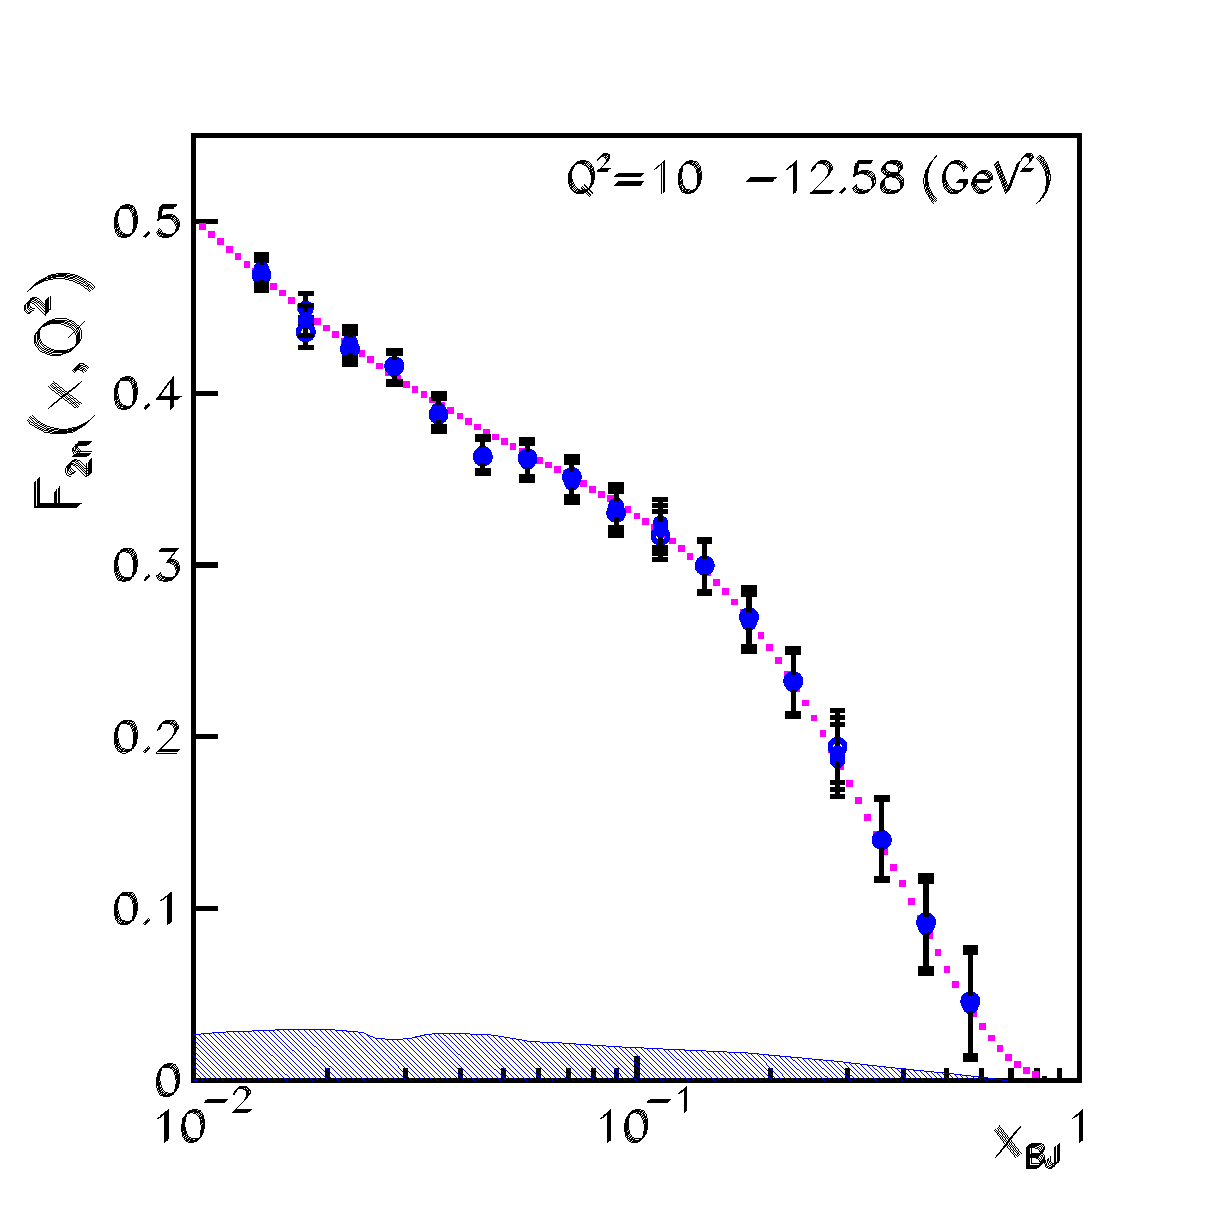
\includegraphics[width=0.55\textwidth]{./LDRD2015/q2_11p29_extrapolated_f2n_vs_xbj_with_syserr2.ps}
  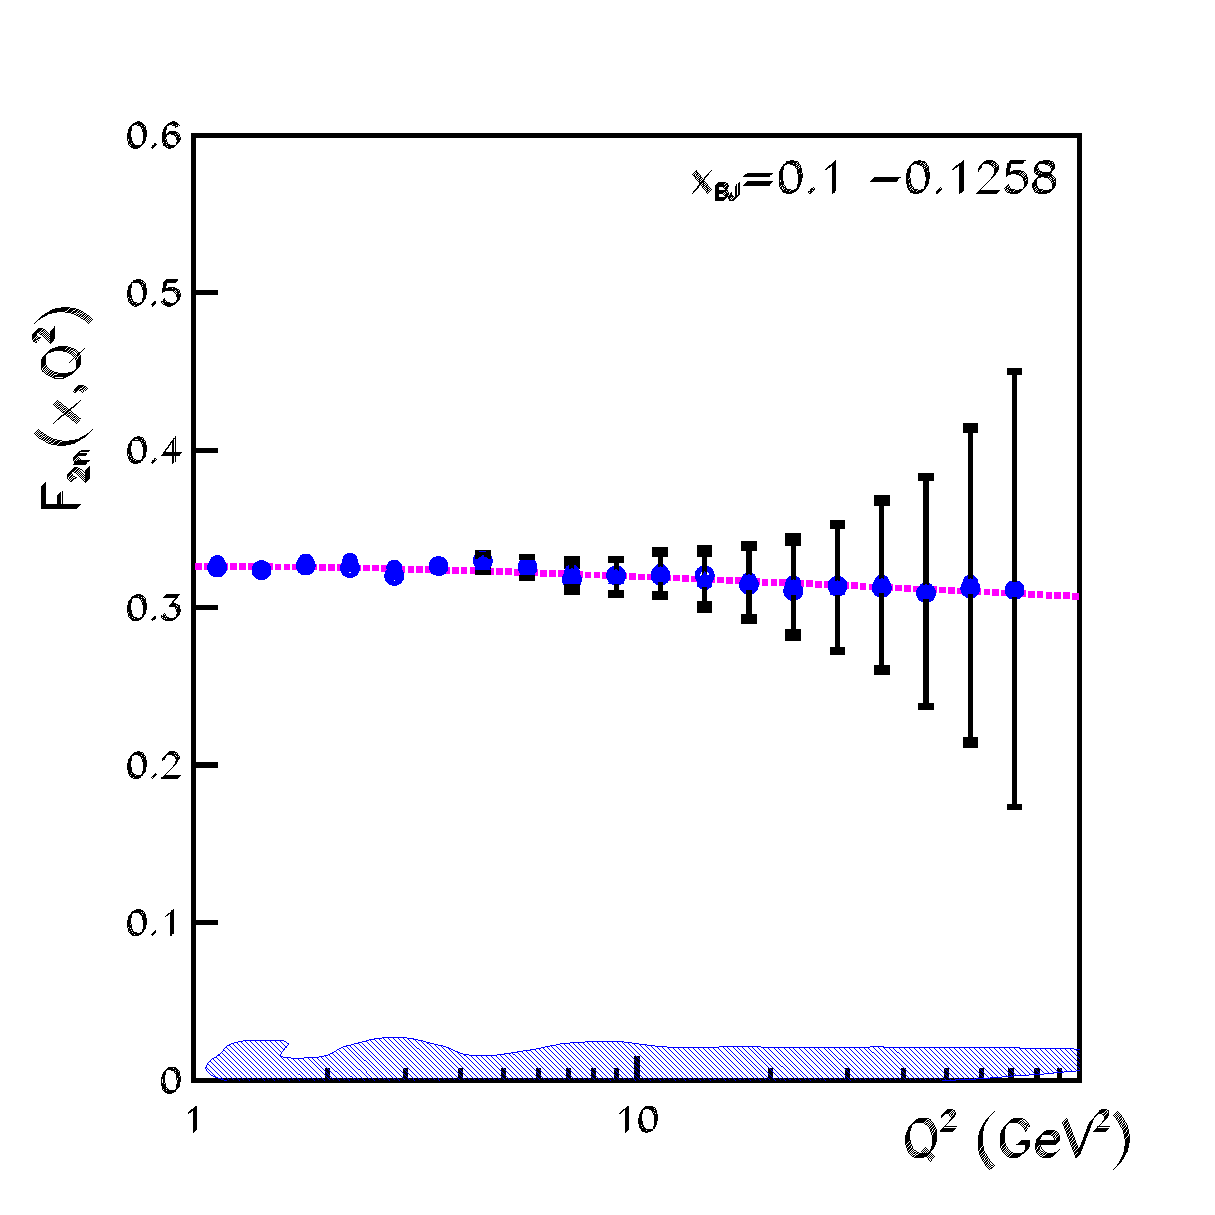
\includegraphics[width=0.55\textwidth]{./LDRD2015/xbj_0p1129_extrapolated_f2n_vs_q2_with_syserr2.ps}
  \caption[On-shell $F_{2n}$]{On-shell $F_{2n}$ as a function of $x_{BJ}$ (Left) at fixed $\langle Q^2 \rangle =11.29$ GeV$^2$, $Q^2$ (Right) at fixed $\langle x_{BJ} \rangle =0.1129$. The magenta dots represent the $F_{2n}$ from model input. The blue shade band on the bottom shows the systematic uncertainty. \label{fig:F2NExtra2}}
\end{figure}

     

\subsection{Polarized ($\vec{e}, \vec{D}$) for $A_{||}$ $(x, Q^2, \alpha_R, -t^{\prime})$}

 Asymmetry ($A^n_{||}$) and depolarization ($D^{\prime}$) factor are defined in Eq.~(\ref{eq:asym}).
\begin{eqnarray}\label{eq:asym}
A^n_{||} = \left(\frac{N_+ - N_-}{N_+ + N_-}\right),~\delta A = \sqrt{\frac{1-A^2}{N_+ + N_-}}
~{\rm{and}}~D^{\prime} =\frac{(1-\epsilon)(2-y)}{y(1+\epsilon R)}
\end{eqnarray}
 ~where, $N_{\pm}$ is the number of cross-section weighted event in each helicity state ($hel=\pm1$) along each beam, $y = Q^2/x_D/(s_{eD}-M_D^2)$, and $R = \sigma_L/\sigma_T$. An example of on-shell extrapolation $A_{||}$ in given $x_{BJ}$, $Q^2$ bin is shown in Fig.~\ref{fig:A11Extra}. Asymmetry shows a trivial $-t^{\prime}$ dependence. We used the $1^{st}$ order of polynomial function to fit the data. 
Figure~\ref{fig:A11Extra2} shows examples of $A_{||}$ on-shell extrapolation with various $x_{BJ}$ from $10^{-2}$ to $1$ at fixed $\langle Q^2 \rangle$=11.29 GeV$^2$  (left) and various $Q^2$ from $1$ to $10^2$GeV$^2$ at fixed $\langle x_{BJ} \rangle$ =0.1129 (right). On right side of each plot, we also show the absolute difference of $A_{||}$ between model input and simulation.
\begin{figure}[htb]
  \begin{center} 
    \begin{tikzpicture} 
      \node[anchor=south west,inner sep=0pt] at (-0.7,-1.7) {\includegraphics[width=0.6\textwidth]{./LDRD2015/cw_asymmetry_weight_fit3comp_x_001_002.ps}};
      \draw[red,ultra thick,rounded corners] (1.5,1.6) rectangle (1.3,0.7);
    \end{tikzpicture}
    \caption{$A_{||}$ fit with $1^{st}$ order of polynomial function in terms of $-t^{\prime}$ to extrapolate to on-shell point. Symbols are same as Fig.~\ref{fig:F2NExtra}.
      \label{fig:A11Extra}
    }
  \end{center} 
\end{figure}





\begin{figure}[htb]
  \hspace{-12mm}
  \includegraphics[width=0.55\textwidth]{./LDRD2015/q2_11p29_extrapolated_asym_vs_xbj_with_error2.ps}
  \includegraphics[width=0.55\textwidth]{./LDRD2015/x_0p1129_extrapolated_asym_vs_q2_with_error2.ps}
  \caption[On-shell $A_{||}$]{On-shell $A_{||}$ extrapolation as a function of $x_{BJ}$ (Left) at fixed $\langle Q^2 \rangle =11.29$ GeV$^2$, $Q^2$ (Right) at fixed $\langle x_{BJ} \rangle =0.1129$\label{fig:A11Extra2}}
\end{figure}
 
%% \subsection{Mapping $F_{2n}$ as a function of $x_{BJ}, Q^2$}

%% \begin{figure}[h]
%%   \begin{center}
%%     \includegraphics[width=0.7\textwidth]{./LDRD2015/x_q2_map_using_cw_f2n_weight.ps}
%%     \caption[Kinematic Mapping]{Kinematic map of $F_{2n}$ ($\hat z$-axis) in terms of $x_{BJ}, Q^2$. Band-(a): $x_{BJ}$ dependence at fixed $Q^2=10.0-12.58$ GeV$^2$, band-(b): $Q^2$ dependence at fixed $x_{BJ}=0.1-0.126$ }
%%   \end{center}
%% \end{figure} 

In figure~\ref{fig:F2NExtra2} and ~\ref{fig:A11Extra2}, we take into account followings:
\begin{itemize}
\item A 10\% uncertainty in the intrinsic momentum spread of deuteron beam ($\delta p/p = 0.1$) is the major systematic uncertainty.
\item This systematic uncertainty is dominated at lower $-t^{\prime}$.
\item Analyses with two $\alpha_R$ cuts show a consistent result of extrapolation. 
\item A full grid scan of $x_{BJ}$ and $Q^2$ dependent (un)polarized neutron structure functions ($F_{2n}$, $A_{||}$) allows us to estimate an evolution of global PDFs uncertainty.
\end{itemize}

\section{Event display with GEMC detector}\label{GEMC_Detector}
Independently, a detector software group is developing the detector simulation program in the GEANT4 framework, so called GEant Monte-Carlo (GEMC)~\cite{EIC_GEMC}. Our event generator produces the output with same format of GEMC that directly be used as a GEMC input. Figure~\ref{fig:STEGGEMC} shows an example of event display snapshot through GEMC. Figure top shows the current design of JLab version EIC beam line and detector components (for now it displays only a dual solenoid magnet) in the first interaction point (IP1). It shows 50 events of scattered electrons (blue rays) and spectator protons (red rays). Other detector components are inactivated in this figure for the tracking view purpose. On the bottom side plot shows the acceptance as functions of $p_T$, $\alpha_R$. Here, the acceptance is calculated by  the number of event passed the second dipole over the number of generated. As it shown, the acceptance drops at smaller $\alpha_R$ because lower momentum spectator protons barely pass the second dipole. Note that $\alpha_R$ goes the same way with bending spectator proton at the second dipole.
\begin{figure}
%  \hspace{-8mm}
\begin{center}
    \includegraphics[angle=0,width=0.6\textwidth]{./LDRD2015/GEMC_IP1_STEGp_WideKine_evt50.ps}\\
    %% \includegraphics[angle=0,width=0.55\textwidth]{./LDRD2015/pT_alpah_D2exit.eps}
    \includegraphics[angle=0,width=0.7\textwidth]{./LDRD2015/alpha_vs_pT.ps}
    \caption[STEG event with GEMC]{Top: JLab EIC beam-line with spectator proton (red rays) and scattered electrons (blue rays), Bottom: Acceptance as function of $p_T$, $\alpha_R$ at the exit of the second dipole. 
    \label{fig:STEGGEMC}
        }
\end{center}
\end{figure}






\section{Summary}
 We have developed a MC simulation of Spectator tagging event generator with (M)EIC configuration. 
Again, overview of this project and more detail information are available on the public project web-page at \url{https://www.jlab.org/theory/tag/}. All current version of computer codes, documentation, background information are also available in this web-site.

A spectator tagging technique using (un)polarized deuteron and electron beams allows us to measure (un)polarized neutron structure under controlled uncertainty and model-independently.
Using this method, on-shell extrapolation of $F_{2n}$ and $A^n_{||}$ have been carried out using our pseudo-data.
Overall, a \% level of statistical uncertainty is achievable in given luminosity, but the systematical uncertainty is dominated due to the uncertainty in the intrinsic momentum spread of deuteron beam.
 We estimated the global systematic uncertainty $\delta \sigma/\sigma$ = 2.5\% for unpolarized cross-sections and $\delta A/A$ = 1.7\% for raw asymmetries.  
 Our point-to-point systematic uncertainty is calculated by taking a Gaussian randomization into account and is about 0.5\%.
We look forward to seeing what these pseudo-data can guide for the global fits.  



%% \begin{itemize}
%% \item We have established the MC simulation with (M)EIC configuration\\
%%   - Public project web-page at \url{https://www.jlab.org/theory/tag/}\\
%%   - Computer codes, documentation, background information, links
%% \item Spectator tagging allows to measure (un)polarized neutron structure under controlled uncertainty and model-independently\\ 
%%   - On-shell extrapolation of $F_{2n}$ \& $A^n_{||}$ have been obtained\\ 
%%   - Overall 1\% level of statistical uncertainty, but dominant uncertainty is the systematical uncertainty\\ 
%%   - Global systematic uncertainty $\delta \sigma/\sigma$ = 2.5\%, $\delta A/A$ = 1.7\%\\ 
%%   - Point-to-point systematic uncertainty (Gaussian randomization) $\sim$ 0.5\% 
%% \item Looking forward to seeing what pseudo-data can guide for the global fits
%% \end{itemize}



















\begin{thebibliography}{0}
\bibitem{MSargsian} \small{M.~Sargsian and M.~Strikman, ``Model independent method for determination of the DIS structure of free neutron'', Phys. Lett. B \textbf{639}, 223 (2006).}
\bibitem{CWeiss2014} \small{C.~Weiss {\em et al.}, ``Physics potential of polarized light ions with EIC at JLab'', Laboratory Directed Research and Development Proposal, (2014).}
%%\bibitem{gitHubLink} \small{~\url{https://github.com/JeffersonLab/LightIonEIC/releases/tag/v0.1}}
\bibitem{gitHubLink} \small{~\url{https://github.com/JeffersonLab/LightIonEIC/releases/tag/v0.2}}

\bibitem{JLabtheoryWeb} \small{JLab theory website for Spectator Tagging Project, \url{https://www.jlab.org/theory/tag/}}
\bibitem{LundWeb} \small{EIC GEMC I/O format,~\url{https://gemc.jlab.org/gemc/Documentation/Entries/2011/3/18_The_LUND_Format.html}}
\bibitem{EIC_GEMC} \small{EIC Detector Software Simulation (GEMC),~\url{https://eic.jlab.org/wiki/index.php/EIC_Detector_Software_Simulation}}
%% \bibitem{Pedro2014} P.~Jimenez-Delgado, E.~Reya, Phys.~Rev.~D\textbf{89} 074049, (2014).

\end{thebibliography}



\end{document}

 
